%!TEX root=../../main.tex

\paragraph{OR'2014} This appendix contains the paper submitted to the $9^{th}$
International Conference on Open Repositories (OR'2014), taking place in
Helsinki, Finland. It is the leading conference in its field, with hundreds of
participants from all around the world. The website of the conference is
\url{http://or2014.helsinki.fi/}.

Note that this paper was authored approximately two months before the end of
the project, and thus, certain details might be missing or inaccurate in
regards to the final state of the deliverable.

Paper follows on next page, the length being of three pages.

\paragraph{AAHEP7} A presentation regarding the annotation developments in
Invenio will be given by Dr. Tibor \v{S}imko at the $7^{th}$ Summit of
Information Providers in Astronomy, Astrophysics and High Energy Physics. This
summit is attended by representatives of organisations providing access to
information in these fields, such as INSPIRE, ADS, or arXiv, and will take
place at the Stony Brook University, Stony Brook, New York, United States of
America, between 1--3 April, 2014. The event's website is
\url{http://indico.cern.ch/event/262430/}.

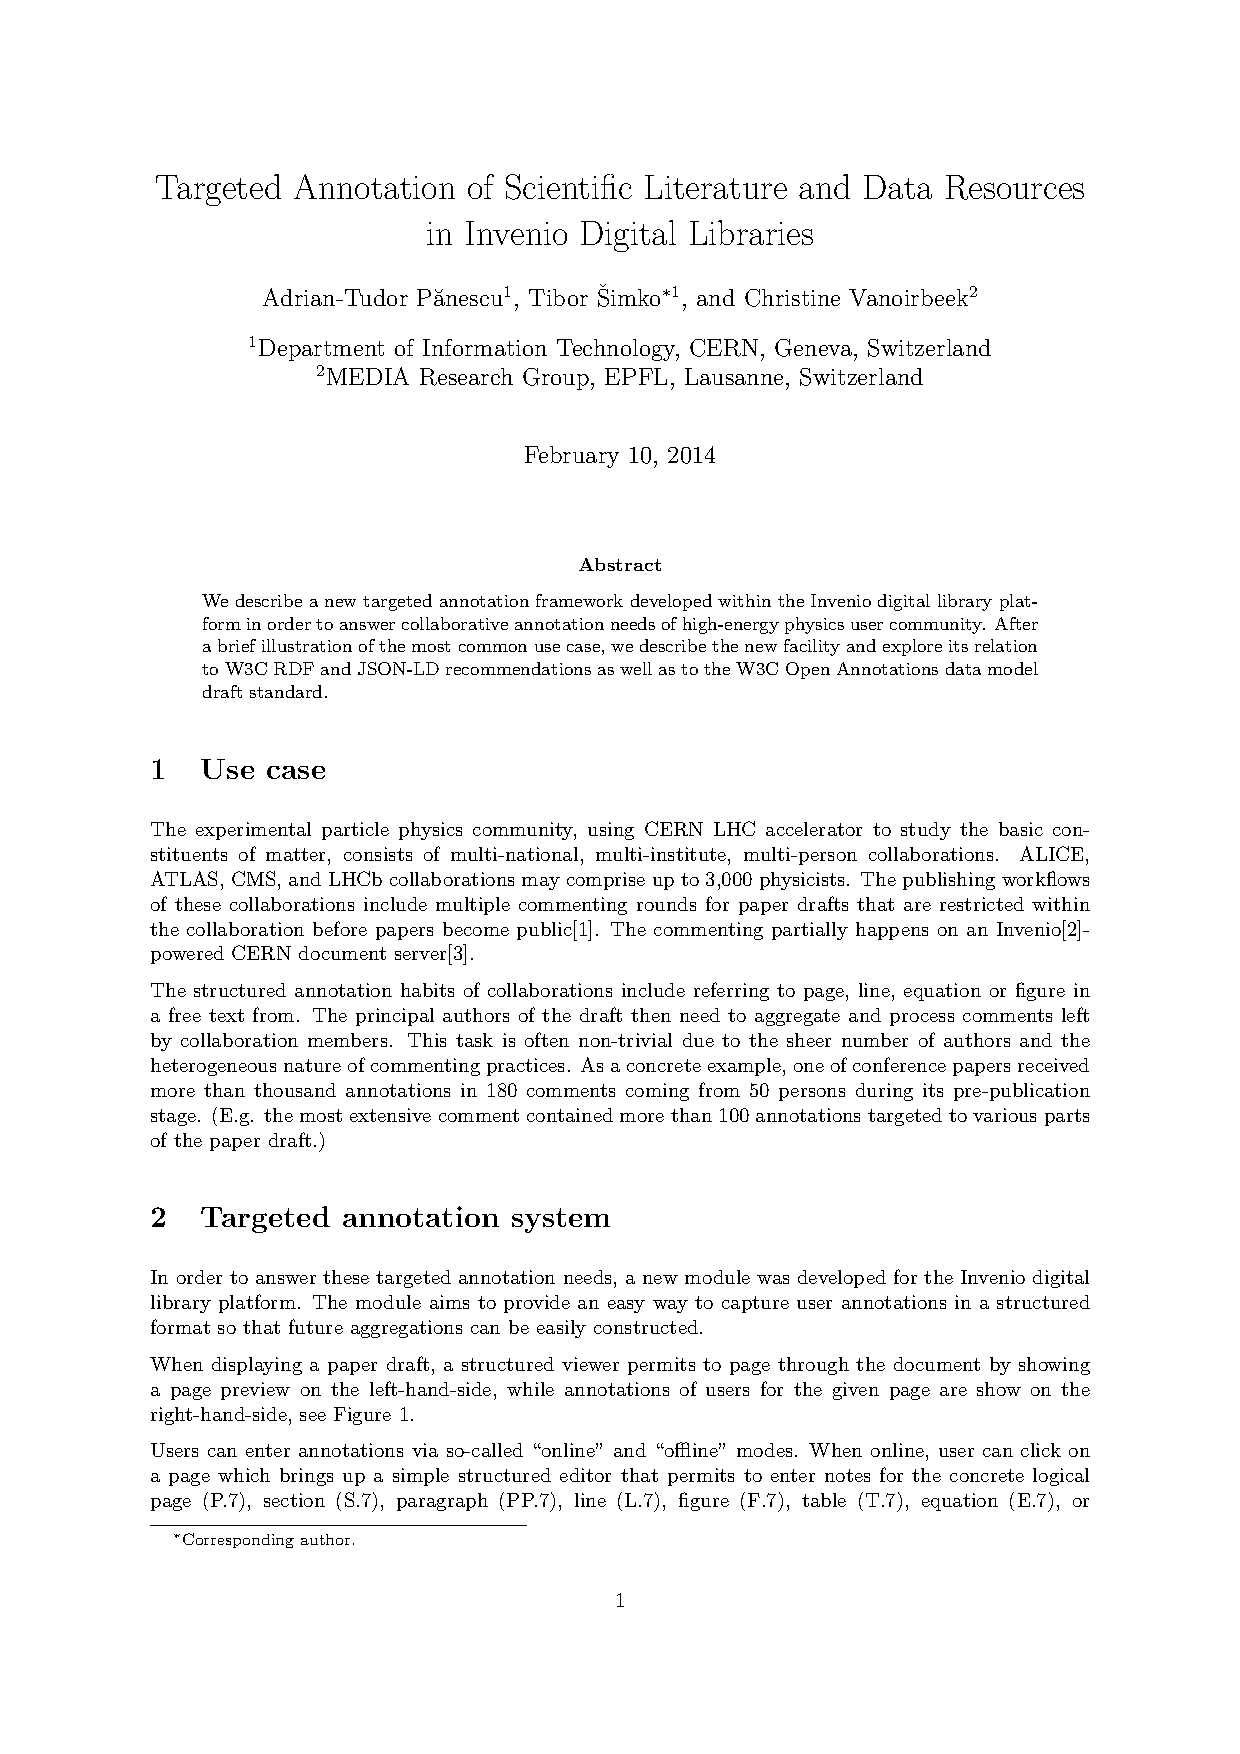
\includepdf[pages={1-3}]{static/pdf/or2014-invenio-annotations.pdf}
